\newpage
\subsection{Caso d'uso UC1: Registrazione}
\begin{figure}[h] 
	\centering 
	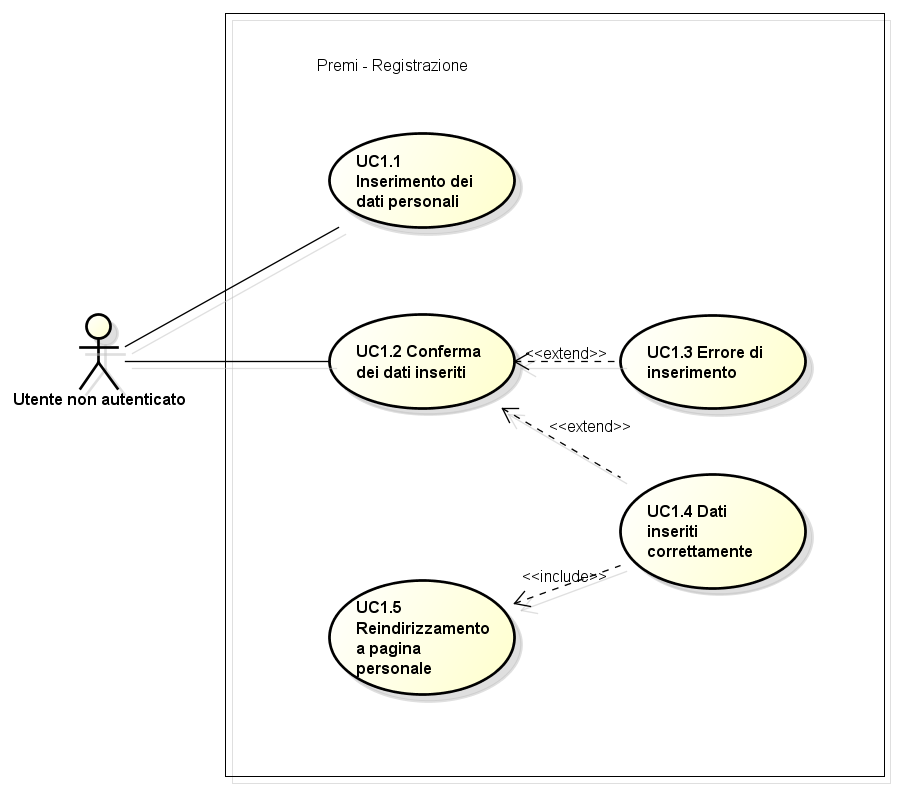
\includegraphics[scale=0.45] {img/UC1.png} 
	\caption{UC1 - Registrazione} 
\end{figure}

\begin{itemize}
	\item \textbf{Attori:} Utente non autenticato;
	\item \textbf{Scopo e descrizione:} L'utente non è iscritto e vuole avviare la procedura di iscrizione al sito;
	\item \textbf{Precondizione:} L'utente ha selezionato la voce "registrati" presente sul sito;
	\item \textbf{Flusso principale degli eventi:}
	\begin{enumerate}
		\item L'utente inserisce i propri dati personali [UC1.1];
		\item L'utente conferma l'inserimento dei propri dati [UC1.2];
		\item Si può verificare un errore di inserimento [UC1.3];
		\item I dati sono stati inseriti correttamente [UC1.4];
		\item Il sistema reindirizza l'utente alla sua pagina personale [UC1.5];
	\end{enumerate}
	\item \textbf{Postcondizione:} Il sistema ha registrato il nuovo utente e lo ha reindirizzato alla propria pagina personale.
\end{itemize}

\newpage

\subsection{Caso d'uso UC1.1: Inserimento dati personali}
\begin{figure}[h] 
	\centering 
	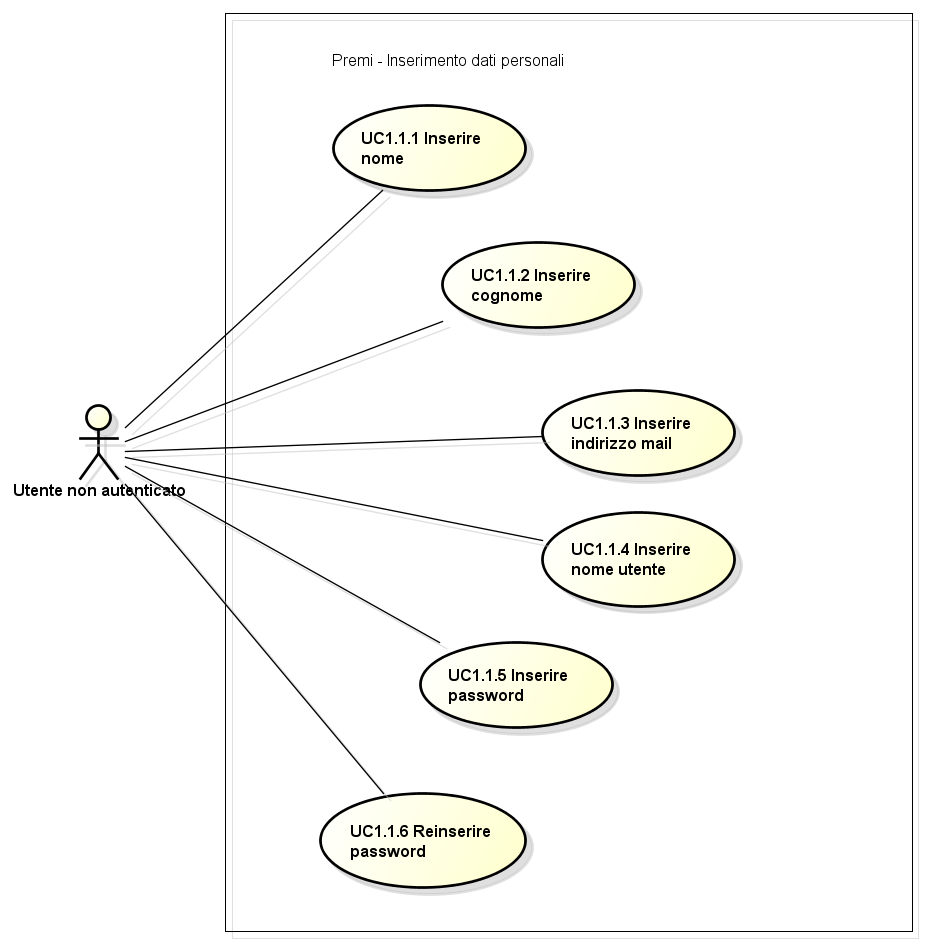
\includegraphics[scale=0.45] {img/UC1.1.png} 
	\caption{UC1.1 - Inserimento dati personali} 
\end{figure}
\begin{itemize}
	\item \textbf{Attori:} Utente non autenticato;
	\item \textbf{Scopo e descrizione:} L'utente inserisce tutti i dati richiesti per la registrazione;
	\item \textbf{Precondizione:} L'utente visualizza la schermata di inserimento dei dati richiesti per la registrazione;
	\item \textbf{Flusso principale degli eventi:}
	\begin{enumerate}
		\item L'utente inserisce il proprio nome [UC1.1.1];
		\item L'utente inserisce il proprio cognome [UC1.1.2];
		\item L'utente inserisce il proprio indirizzo mail [UC1.1.3];
		\item L'utente inserisce il proprio nome utente [UC1.1.4];
		\item L'utente inserisce una password [UC1.1.5];
		\item L'utente inserisce nuovamente la password [UC1.1.6].
	\end{enumerate}
	\item \textbf{Postcondizione:} Tutti i campi richiesti sono stati compilati correttamente.
\end{itemize}

\subsection{Caso d'uso UC1.1.1: Inserire nome}
\begin{itemize}
	\item \textbf{Attori:} Utente non autenticato;
	\item \textbf{Scopo e descrizione:} L'utente inserisce il proprio nome;
	\item \textbf{Precondizione:} La casella dove inserire il nome è vuota;
	\item \textbf{Postcondizione:} La casella è stata compilata con il nome inserito dall'utente.
\end{itemize}

\subsection{Caso d'uso UC1.1.2: Inserire cognome}
\begin{itemize}
	\item \textbf{Attori:} Utente non autenticato;
	\item \textbf{Scopo e descrizione:} L'utente inserisce il proprio cognome;
	\item \textbf{Precondizione:} La casella dove inserire il cognome è vuota;
	\item \textbf{Postcondizione:} La casella è stata compilata con il cognome inserito dall'utente.
\end{itemize}

\subsection{Caso d'uso UC1.1.3: Inserire indirizzo mail}
\begin{itemize}
	\item \textbf{Attori:} Utente non autenticato;
	\item \textbf{Scopo e descrizione:} L'utente inserisce il proprio indirizzo mail;
	\item \textbf{Precondizione:} La casella dove inserire l'indirizzo mail è vuota;
	\item \textbf{Postcondizione:} La casella è stata compilata con l'indirizzo mail inserito dall'utente.
\end{itemize}

\subsection{Caso d'uso UC1.1.4: Inserire nome utente}
\begin{itemize}
	\item \textbf{Attori:} Utente non autenticato;
	\item \textbf{Scopo e descrizione:} L'utente inserisce il proprio nome utente;
	\item \textbf{Precondizione:} La casella dove inserire il nome utente è vuota;
	\item \textbf{Postcondizione:} La casella è stata compilata con il nome utente inserito dall'utente.
\end{itemize}

\subsection{Caso d'uso UC1.1.5: Inserire password}
\begin{itemize}
	\item \textbf{Attori:} Utente non autenticato;
	\item \textbf{Scopo e descrizione:} L'utente inserisce la propria password;
	\item \textbf{Precondizione:} La casella dove inserire la password è vuota;
	\item \textbf{Postcondizione:} La casella è stata compilata con la password inserita dall'utente.
\end{itemize}

\subsection{Caso d'uso UC1.1.6: Reinserire password}
\begin{itemize}
	\item \textbf{Attori:} Utente non autenticato;
	\item \textbf{Scopo e descrizione:} L'utente inserisce nuovamente la password inserita in precedenza;
	\item \textbf{Precondizione:} La casella dove inserire la password è già stata compilata e la casella dove reinserire per la seconda volta la password è vuota;
	\item \textbf{Postcondizione:} La casella di reinserimento password è stata compilata con la password inserita dall'utente.
\end{itemize}

\subsection{Caso d'uso UC1.2: Conferma dei dati inseriti}
\begin{itemize}
	\item \textbf{Attori:} Utente non autenticato;
	\item \textbf{Scopo e descrizione:} L'utente deve confermare i dati inseriti in precedenza per procedere con l'iscrizione;
	\item \textbf{Precondizione:} L'utente ha inserito i dati richiesti per la registrazione;
	\item \textbf{Postcondizione:} Il sistema elabora i dati e registra il nuovo utente.
\end{itemize}

\subsection{Caso d'uso UC1.3: Errore di inserimento}
\begin{itemize}
	\item \textbf{Attori:} Sistema;
	\item \textbf{Scopo e descrizione:} Dopo che l'utente ha confermato i dati, il sistema segnala all'utente che c'è stato un errore di inserimento e mostra nuovamente la schermata di inserimento dei dati personali;
	\item \textbf{Precondizione:} L'utente ha confermato i dati inseriti;
	\item \textbf{Postcondizione:} Il sistema segnala all'utente che c'è stato un errore di inserimento e mostra di nuovo la schermata di inserimento dei dati personali.
\end{itemize}

\subsection{Caso d'uso UC1.4: Dati inseriti correttamente}
\begin{itemize}
	\item \textbf{Attori:} Sistema;
	\item \textbf{Scopo e descrizione:} Dopo che l'utente ha confermato i dati inseriti, il sistema li controlla e li accetta e invia una mail di conferma all'utente;
	\item \textbf{Precondizione:} L'utente ha confermato i dati inseriti;
	\item \textbf{Postcondizione:} Il sistema controlla e accetta i dati inseriti dall'utente. Inoltre invia una mail di conferma della registrazione all'utente.
\end{itemize}

\subsection{Caso d'uso UC1.5: Reindirizzamento a pagina personale}
\begin{itemize}
	\item \textbf{Attori:} Sistema;
	\item \textbf{Scopo e descrizione:} Dopo aver confermato i propri dati, il sistema reindirizza l'utente alla propria pagina personale dove può accedere alle varie funzionalità del sito;
	\item \textbf{Precondizione:} Il sistema ha registrato correttamente il nuovo utente;
	\item \textbf{Postcondizione:} Il sistema permette all'utente di visualizzare la propria pagina personale.
\end{itemize}